% ------ IPP overview figure
\begin{figure*}[t]

\begin{tikzpicture}
\node[inner sep=0pt] (overview) at (-2,0) {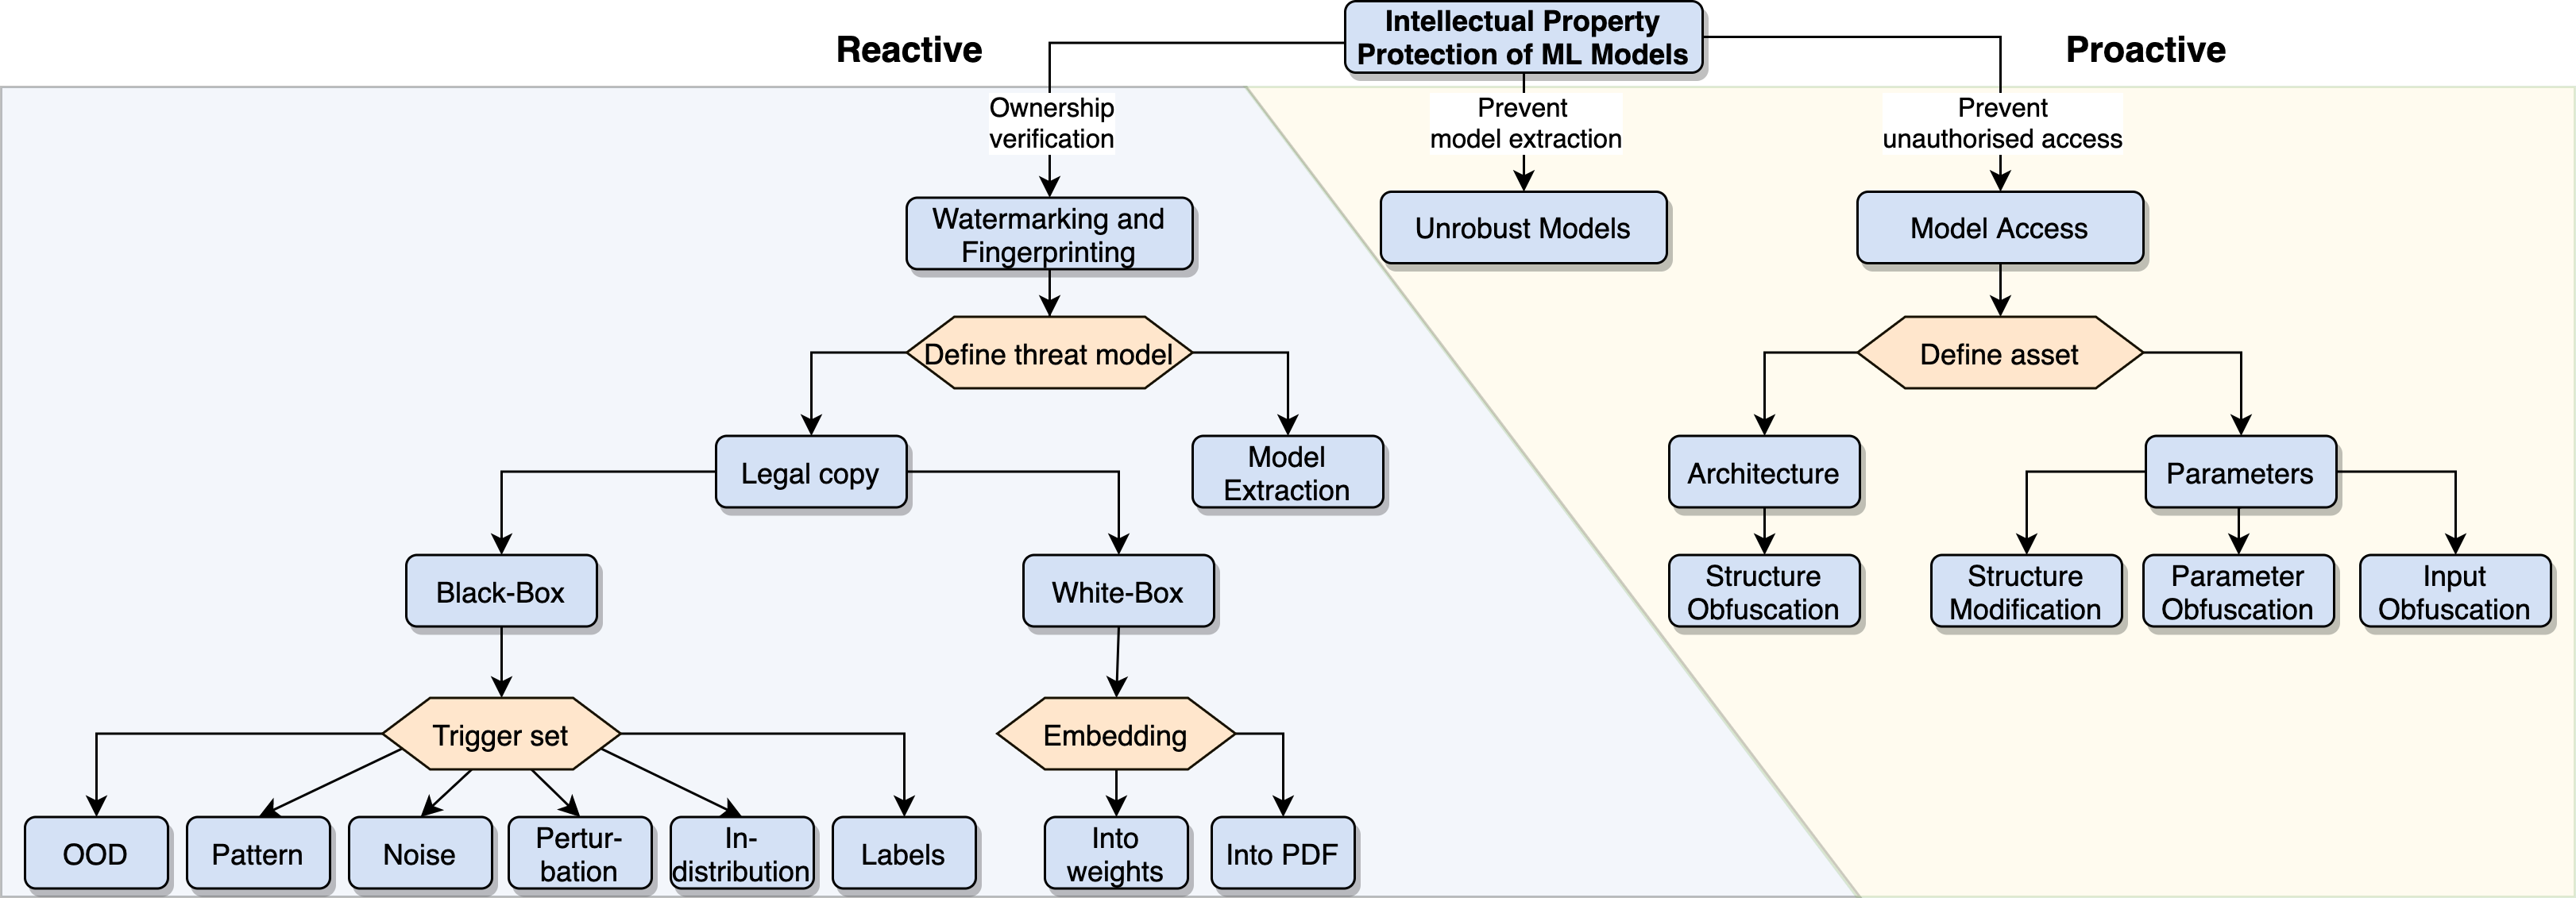
\includegraphics[width=\linewidth]{images/IPP_overview.png}};
%OOD:
\node[inner sep=0pt] (cite1) at (-8.8,-2.7) {\tiny \cite{adi_turning_2018}};
\node[inner sep=0pt] (cite2) at (-8.8,-3) {\tiny \cite{zhang_protecting_2018}};
\node[inner sep=0pt] (cite22) at (-8.8,-3.2) {\tiny \cite{yang_effectiveness_2019}};
%pattern:
\node[inner sep=0pt] (cite3) at (-7.9,-2.7) {\tiny \cite{zhang_protecting_2018}};
\node[inner sep=0pt] (cite4) at (-7.9,-3) {\tiny \cite{li_piracy_2020}};
\node[inner sep=0pt] (cite5) at (-7.9,-3.3) {\tiny \cite{guo_watermarking_2018}};
\node[inner sep=0pt] (cite6) at (-7.9,-3.6) {\tiny \cite{guo_evolutionary_2019}};
%noise:
\node[inner sep=0pt] (cite7) at (-7,-2.7) {\tiny \cite{zhang_protecting_2018}};
\node[inner sep=0pt] (cite8) at (-7,-3) {\tiny \cite{zhu_secure_2020}};
%perturbation:
\node[inner sep=0pt] (cite9) at (-6.05,-2.7) {\tiny \cite{merrer_adversarial_2019}};
\node[inner sep=0pt] (cite10) at (-6.05,-3) {\tiny \cite{li_how_2019}};
\node[inner sep=0pt] (cite11) at (-6.05,-3.3) {\tiny \cite{chen_blackmarks_2019}};
\node[inner sep=0pt] (cite13) at (-6.05,-3.6) {\tiny FP: \cite{lukas_deep_2020}};
\node[inner sep=0pt] (cite12) at (-6.05,-3.9) {\tiny FP: \cite{zhao_afa_2019}};

%in-distr.:
\node[inner sep=0pt] (cite14) at (-5.1,-2.7) {\tiny \cite{namba_robust_2019}};
%trigger labels:
\node[inner sep=0pt] (cite15) at (-4.15,-2.7) {\tiny \cite{lauw_protecting_2020}};
\node[inner sep=0pt] (cite16) at (-4.15,-3) {\tiny \cite{zhang_deeptrigger_2020}};
\node[inner sep=0pt] (cite16) at (-4.15,-3.3) {\tiny \cite{xu_identity_2020}};

%into weights:
\node[inner sep=0pt] (cite17) at (-3,-2.7) {\tiny \cite{uchida_embedding_2017}};
\node[inner sep=0pt] (cite18) at (-3,-3) {\tiny \cite{wang_robust_2020}};
\node[inner sep=0pt] (cite19) at (-3,-3.3) {\tiny \cite{wang_watermarking_2020}};
\node[inner sep=0pt] (cite20) at (-3,-3.6) {\tiny \cite{li_watermarking_2020}};
%into pdf:
\node[inner sep=0pt] (cite21) at (-2,-2.7) {\tiny \cite{rouhani_deepsigns_2019}};
\node[inner sep=0pt] (cite22) at (-2,-3) {\tiny FP: \cite{chen_deepmarks_2019}};
%Model Extraction:
\node[inner sep=0pt] (cite23) at (-2,-0.5) {\tiny \cite{jia_entangled_2020}}; 
\node[inner sep=0pt] (cite24) at (-2,-0.8) {\tiny \cite{szyller_dawn_2020}};
% man könnte noch diese hinzufügen, aber lasse ich für die version erstmal...
%\node[inner sep=0pt] (cite241) at (1.6,-1.4) {\tiny \cite{wu_watermarking_2020}};
%\node[inner sep=0pt] (cite242) at (1.9,-1.4) {\tiny \cite{zhang_model_2020}};

% Unrobust models
 \node[inner sep=0pt] (cite25) at (-0.65,0.85) {\tiny \cite{arai_preventing_2020}};
 
%Structure Obfuscation:
\node[inner sep=0pt] (cite101) at (0.7,-1.2) {\tiny \cite{xu_deepobfuscation_2018}};
 
% Structure Modification:
\node[inner sep=0pt] (cite102) at (2.2,-1.2) {\tiny \cite{fan_rethinking_2019}};

% Parameter Encryption & Obfuscation:
\node[inner sep=0pt] (cite103) at (3.45,-1.2) {\tiny \cite{gomez_security_2019}};
\node[inner sep=0pt] (cite104) at (3.45,-1.5) {\tiny \cite{chakraborty_hardware-assisted_2020}};
\node[inner sep=0pt] (cite105) at (3.45,-1.8) {\tiny \cite{alam_deep-lock_2020}};
\node[inner sep=0pt] (cite106) at (3.45,-2.1) {\tiny \cite{tang_deep_2020}};
\node[inner sep=0pt] (cite107) at (3.45,-2.4) {\tiny \cite{lin_chaotic_2020}};

%Input Obfuscation:
\node[inner sep=0pt] (cite108) at (4.7,-1.2) {\tiny \cite{aprilpyone_training_2020}};
\node[inner sep=0pt] (cite109) at (4.7,-1.5) {\tiny \cite{chen_protect_2018}};

\end{tikzpicture}

%    \caption{Taxonomy of IPP protection mechanisms for ML models.}
    \caption{Taxonomy of Intellectual Property Protection mechanisms for Machine Learning models. Note, that not all considered papers are referenced in this diagram.}
        \label{fig:overview}
\end{figure*}
% ------ end
% Ucomment for local usage
% \input{bibliography.bbl}
